\chapter{Parameterliste} \label{ch:Parameterliste}
\begin{table*}[ht]
	\centering
		\begin{tabular}{|cccc|}
		\hline
		\textbf{Parameter} & \textbf{Variable} & \textbf{Wert} & \textbf{Quelle} \\ \hline
		\multicolumn{1}{|c}{Masse Gesamtaufbau (alles)} & \multicolumn{1}{c} {$--$} &  \multicolumn{1}{c} {1,731 kg} & \multicolumn{1}{c|} {Gemessen}  \\ \hline
		\multicolumn{1}{|c}{Masse Ball} & \multicolumn{1}{c} {$m_{S}$} &  \multicolumn{1}{c} {0,3280 kg} & \multicolumn{1}{c|} {Gemessen}  \\ \hline
		\multicolumn{1}{|c}{Masse Motor} & \multicolumn{1}{c} {$m_{M}$} &  \multicolumn{1}{c} {0,0820 kg} & \multicolumn{1}{c|} {Datenblatt}  \\ \hline
		\multicolumn{1}{|c}{Masse omnidirektionales Rad} & \multicolumn{1}{c} {$m_{OW}$} &  \multicolumn{1}{c} {0.0520 kg} & \multicolumn{1}{c|} {Gemessen}  \\ \hline
		\multicolumn{1}{|c}{Masse virtuelles Rad} & \multicolumn{1}{c} {$m_{W}$} &  \multicolumn{1}{c} {0,4020 kg} & \multicolumn{1}{c|} {Gemessen}  \\ \hline
		\multicolumn{1}{|c}{\begin{tabular}[c]{@{}c@{}}Masse Roboterk�rper\\ (mit Motoren/R�der)\end{tabular}}  & \multicolumn{1}{c} {$m_{B}$} & \multicolumn{1}{c} {1,603 kg} & \multicolumn{1}{c|} {Gemessen}\\ \hline
		\multicolumn{1}{|c}{\begin{tabular}[c]{@{}c@{}}Masse Roboterk�rper\\ (ohne Motoren/R�der)\end{tabular}}  & \multicolumn{1}{c} {$m_{B}$} & \multicolumn{1}{c} {1,2010 kg} & \multicolumn{1}{c|} {Gemessen}\\ \hline
		
		\multicolumn{1}{|c}{Radius Ball} & \multicolumn{1}{c} {$r_{S}$} &  \multicolumn{1}{c} {0,0800 m} & \multicolumn{1}{c|} {Datenblatt}  \\ \hline
		\multicolumn{1}{|c}{Radius virtuelles Rad} & \multicolumn{1}{c} {$r_{W}$} &  \multicolumn{1}{c} {0,0300 m} & \multicolumn{1}{c|} {Datenblatt}  \\ \hline
		\multicolumn{1}{|c}{Radius K�rper} & \multicolumn{1}{c} {$r_{B}$} &  \multicolumn{1}{c} {0,0703 m} & \multicolumn{1}{c|} {Gemessen}  \\ \hline
		\multicolumn{1}{|c}{H�he Massenschwerpunkt} & \multicolumn{1}{c} {$l$} &  \multicolumn{1}{c} {0.236 m} & \multicolumn{1}{c|} {SolidEdge}  \\ \hline
		\multicolumn{1}{|c}{H�he K�rper} & \multicolumn{1}{c} {$h$} &  \multicolumn{1}{c} {0.366 m} & \multicolumn{1}{c|} {SolidEdge}  \\ \hline
		
		
		\multicolumn{1}{|c}{Tr�gheitsmoment Ball} & \multicolumn{1}{c} {$I_{S}$} &  \multicolumn{1}{c} {0,0013 $kgm^{2}$} & \multicolumn{1}{c|} {Berechnet}  \\ \hline
		\multicolumn{1}{|c}{Tr�gheitsmoment Rotor} & \multicolumn{1}{c} {$I_{M}$} &  \multicolumn{1}{c} {3.8e-8 $kgm^{2}$} & \multicolumn{1}{c|} {Datenblatt}  \\ \hline
		\multicolumn{1}{|c}{Tr�gheitsmoment omnidirektionales Rad} & \multicolumn{1}{c} {$I_{OW}$} &  \multicolumn{1}{c} {2,34e-5 $kgm^{2}$} & \multicolumn{1}{c|} {Berechnet}  \\ \hline
		
		\multicolumn{1}{|c}{\begin{tabular}[c]{@{}c@{}}Tr�gheitsmoment der virtuellen R�der\\ ($yz$- und $xz$-Ebene)\end{tabular}}  & \multicolumn{1}{c} {$I_{W,yz, xz}$} & \multicolumn{1}{c} {0.00357 $kgm^{2}$} & \multicolumn{1}{c|} {Berechnet}\\ \hline
		
		\multicolumn{1}{|c}{\begin{tabular}[c]{@{}c@{}}Tr�gheitsmoment virtuelles Rad\\ ($xy$-Ebene)\end{tabular}}  & \multicolumn{1}{c} {$I_{W,xy}$} & \multicolumn{1}{c} {0.0143 $kgm^{2}$} & \multicolumn{1}{c|} {Berechnet}\\ \hline
		
		\multicolumn{1}{|c}{\begin{tabular}[c]{@{}c@{}}Tr�gheitsmoment K�rper\\ ($yz$-Ebene)\end{tabular}}  & \multicolumn{1}{c} {$I_{B,yz}$} & \multicolumn{1}{c} {0.0880 $kgm^{2}$} & \multicolumn{1}{c|} {SolidEdge}\\ \hline
		\multicolumn{1}{|c}{\begin{tabular}[c]{@{}c@{}}Tr�gheitsmoment K�rper\\ ($xz$-Ebene)\end{tabular}}  & \multicolumn{1}{c} {$I_{B,xz}$} & \multicolumn{1}{c} {0.0880 $kgm^{2}$} & \multicolumn{1}{c|} {SolidEdge}\\ \hline
		\multicolumn{1}{|c}{\begin{tabular}[c]{@{}c@{}}Tr�gheitsmoment K�rper\\ ($xy$-Ebene)\end{tabular}}  & \multicolumn{1}{c} {$I_{B,xy}$} & \multicolumn{1}{c} {0.0070 $kgm^{2}$} & \multicolumn{1}{c|} {SolidEdge}\\ \hline
		
		\multicolumn{1}{|c}{�bersetzungsverh�ltnis} & \multicolumn{1}{c} {$i$} &  \multicolumn{1}{c} {353,5} & \multicolumn{1}{c|} {Datenblatt}  \\ \hline
		\multicolumn{1}{|c}{Erdbeschleunigung} & \multicolumn{1}{c} {$g$} &  \multicolumn{1}{c} {9,81 $\frac{m}{s^{2}}$} & \multicolumn{1}{c|} {Datenblatt}  \\ \hline
		\end{tabular}
\end{table*}

\chapter{Bestands-Liste}
\begin{table}[H]
	\centering
	\caption{Screws:}
	\label{screws}
	\begin{tabular}{|c|c|c|c|}
		\hline
		{\textbf{Type}} & {\textbf{Size}}                                             & { \textbf{Amount}} & { \textbf{Place}} \\ \hline
		Cylinderhead screw  & M3 x 11mm                                                       & 8                     & Motor mounts         \\ \hline
		Cylinderhead screw  & M2,5 x 22mm                                                     & 16                    & Motor plate          \\ \hline
		Cylinderhead screw  & M2 x 6 mm                                                       & 18                    & Wheel shaft          \\ \hline
		Cylinderhead screw  & \begin{tabular}[c]{@{}c@{}}M2,5  x 36 mm\\ (38 mm)\end{tabular} & 5                     & Wheel shaft cover    \\ \hline
		Cylinderhead screw  & \begin{tabular}[c]{@{}c@{}}M3 x 20 mm\\ (21mm)\end{tabular}     & 4                     & Layer mounting       \\ \hline
		Nut                 & M2                                                              & 5                     & Layer mounting       \\ \hline
		Cylinderhead screw  & \begin{tabular}[c]{@{}c@{}}M2,5 x 22mm\\ (23mm)\end{tabular}    & 4                     & Layer mounting       \\ \hline
	\end{tabular}
\end{table}

\begin{table}[H]
	\centering
	\caption{�bersicht �ber die verwendeten Bauteile}
	\label{bauteile1}
\begin{tabular}{l l l l l}
	Item & \# & W.[g] & Weblink & Bild\\ \hline
	OpenCR Board (Controlling the motors, IMU)&1&60&\mylink{https://github.com/ROBOTIS-GIT/OpenCR/wiki/Hardware_Specification\#specification}{github\_wiki} 
	&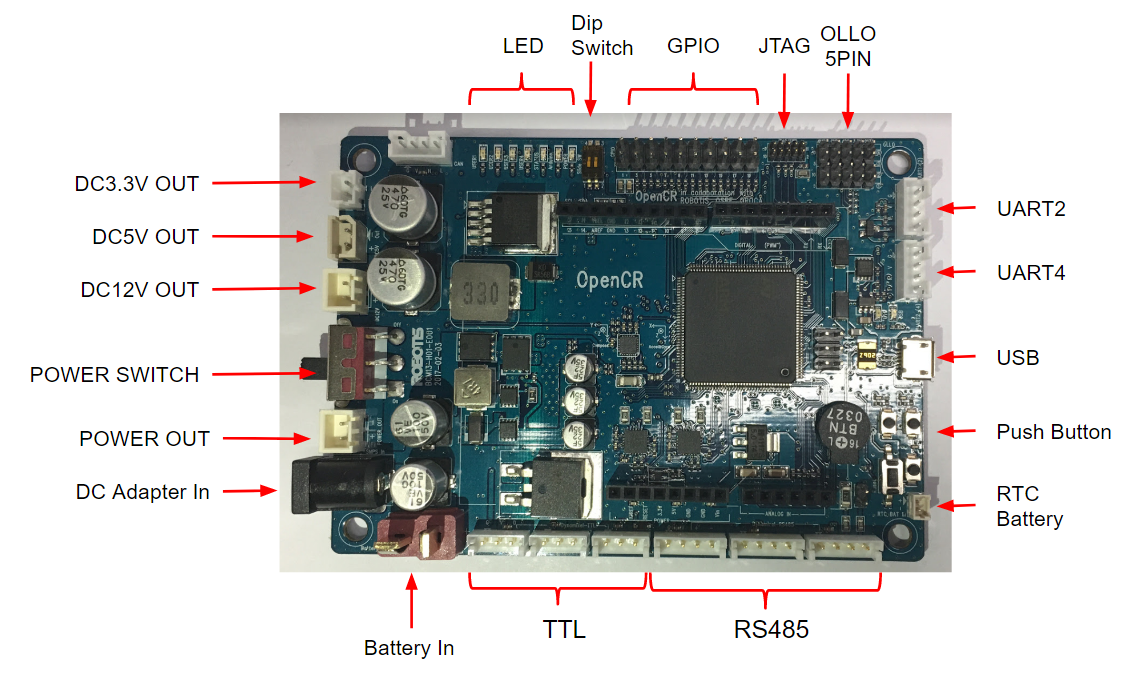
\includegraphics[width=0.1\textwidth]{./Bilder/Markus/img/opencr.png}  \\
		
	UpBoard (Main PC)&1 &96 & \mylink{https://up-shop.org/up-boards/44-up-board-4gb-ram-64-gb-emmc.html}{\EUR{127}}
	&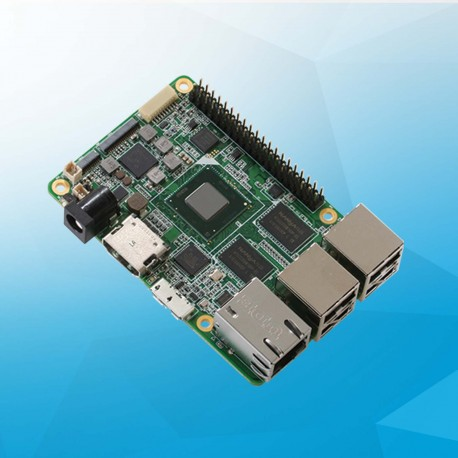
\includegraphics[width=0.1\textwidth]{./Bilder/Markus/img/upboard.jpg} \\
		
	Intel RealSense R200&1& 9.4& \mylink{https://www.intel.de/content/www/de/de/support/articles/000023534/emerging-technologies/intel-realsense-technology.html}{datasheet, \EUR{84.15}}&
	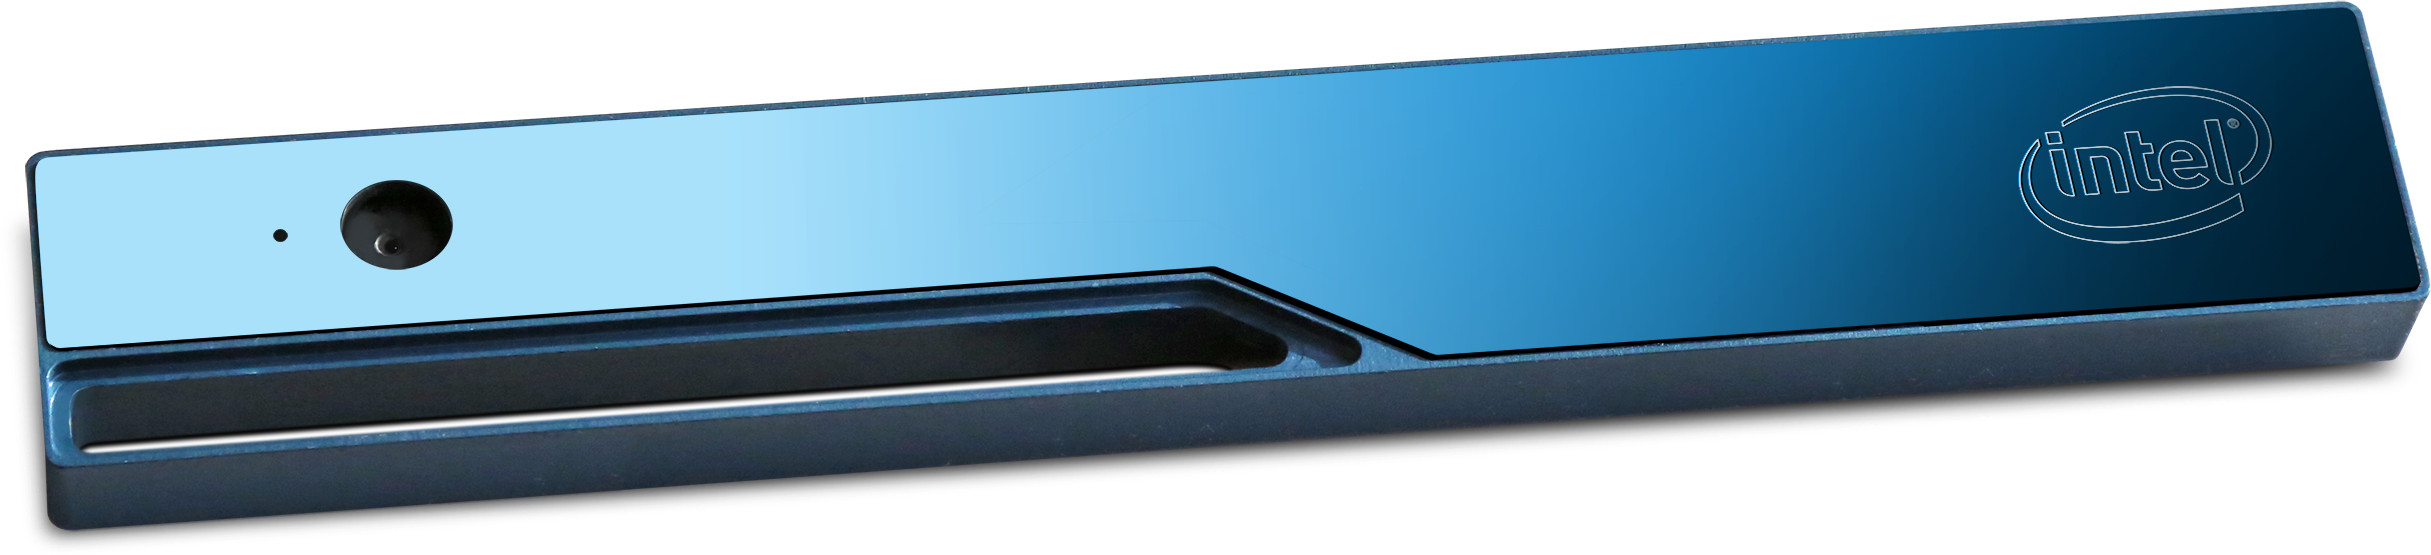
\includegraphics[width=0.1\textwidth]{./Bilder/Markus/img/r200.jpg} \\
\end{tabular}
\end{table}

\begin{table}[]
	\centering
	\caption{�bersicht �ber die verwendeten Bauteile}
	\label{bauteile2}
\begin{tabular}{l l l l l}
	Item & \# & W.[g] & Weblink & Bild\\ \hline
			
			Laser Distance Sensor&1 &124 &\mylink{https://wiki.ros.org/hls_lfcd_lds_driver?action=AttachFile\&do=view\&target=LDS_Basic_Specification.pdf}{specs, \EUR{100}} & 
			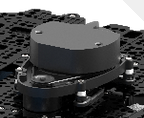
\includegraphics[width=0.1\textwidth]{./Bilder/Markus/img/lasersensor.png}\\
			
			Battery: LI-PO 11.1 1800mAh LB-12 19&1&132 &\mylink{https://nodna.de/Robotis-LIPO-111V-Akkupack-1800mAh-LBS-012}{\EUR{44.90}} &
			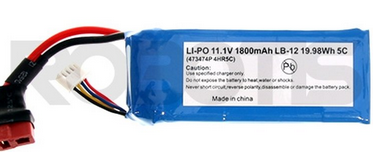
\includegraphics[width=0.1\textwidth]{./Bilder/Markus/img/battery.png} \\
			
			Turtlebot3 Layers(125cmx125cm)&4& & & \\
			
			XM430-W350-R Dynamixel (Motors)&3&82 &\mylink{http://support.robotis.com/en/product/actuator/dynamixel_x/xm_series/xm430-w350.htm}{robotis,\EUR{250}} &
			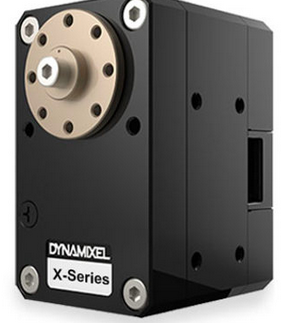
\includegraphics[width=0.1\textwidth]{./Bilder/Markus/img/dynamixel.png}\\ 
			
			Ball(alum., dia.: 140mm, material thickness 2.5mm)&1&400&\mylink{http://www.ball-tech.de/Hohlkugeln/Aluminium/}{ball-tech gmbh,\EUR{40}. } & 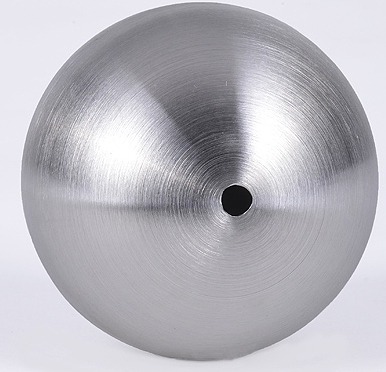
\includegraphics[width=0.1\textwidth]{./Bilder/Markus/img/ball.png}\\
			
			Omni wheels(dia: 60mm, thickness:25mm)&3&51.46 &\mylink{http://krause-robotics.de/xtshop/Antriebe/Raeder/Allseitenraeder/Allseitenraeder-60-mm:::99_100_106_114.html}{\EUR{10.38}}&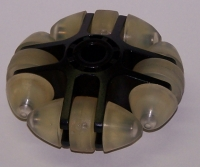
\includegraphics[width=0.1\textwidth]{./Bilder/Markus/img/wheel.jpg}   \\
			
			Kreisring (PLA, 3D printeted)&1&28 & & 
			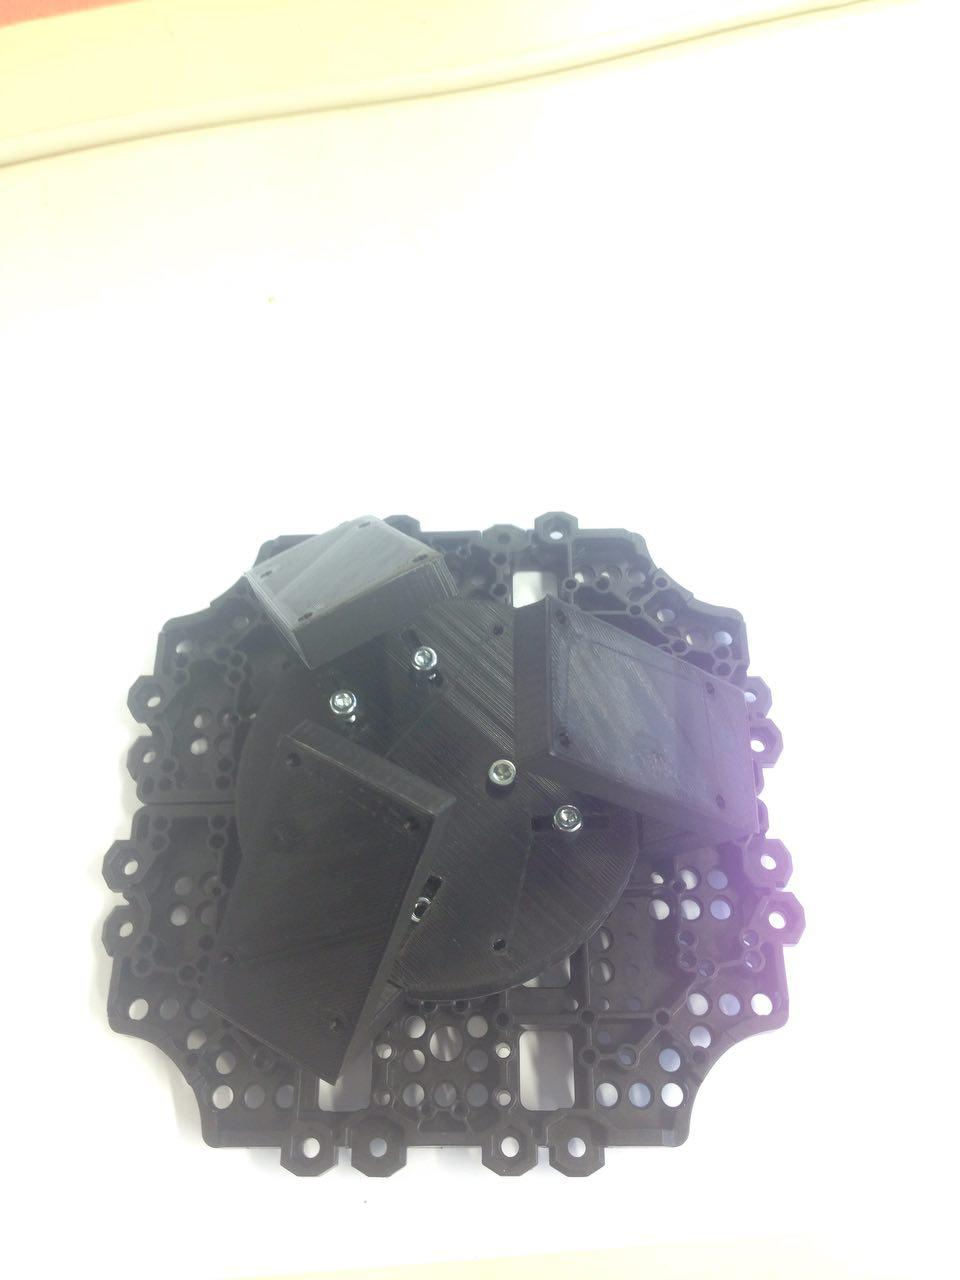
\includegraphics[width=0.1\textwidth]{./Bilder/Markus/img/kreisring.png}\\
			
			Halterung (PLA, 3D printeted)&3&18 & & 
			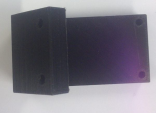
\includegraphics[width=0.1\textwidth]{./Bilder/Markus/img/halterung.png} \\
			
			Mitnehmer (PLA, 3D printeted)&3&8 & &
			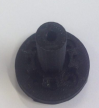
\includegraphics[height=0.06\textwidth]{./Bilder/Markus/img/mitnehmer.png}  \\
			
			Plain washer (Beilagscheibe),(PLA, 3D printeted)&3&0.45 & &
			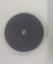
\includegraphics[height=0.06\textwidth]{./Bilder/Markus/img/beilagscheibe.png}  \\
			
			Omni double wheels(dia: 56mm, thickness:25mm)&3&62 &{\EUR{15}} &  	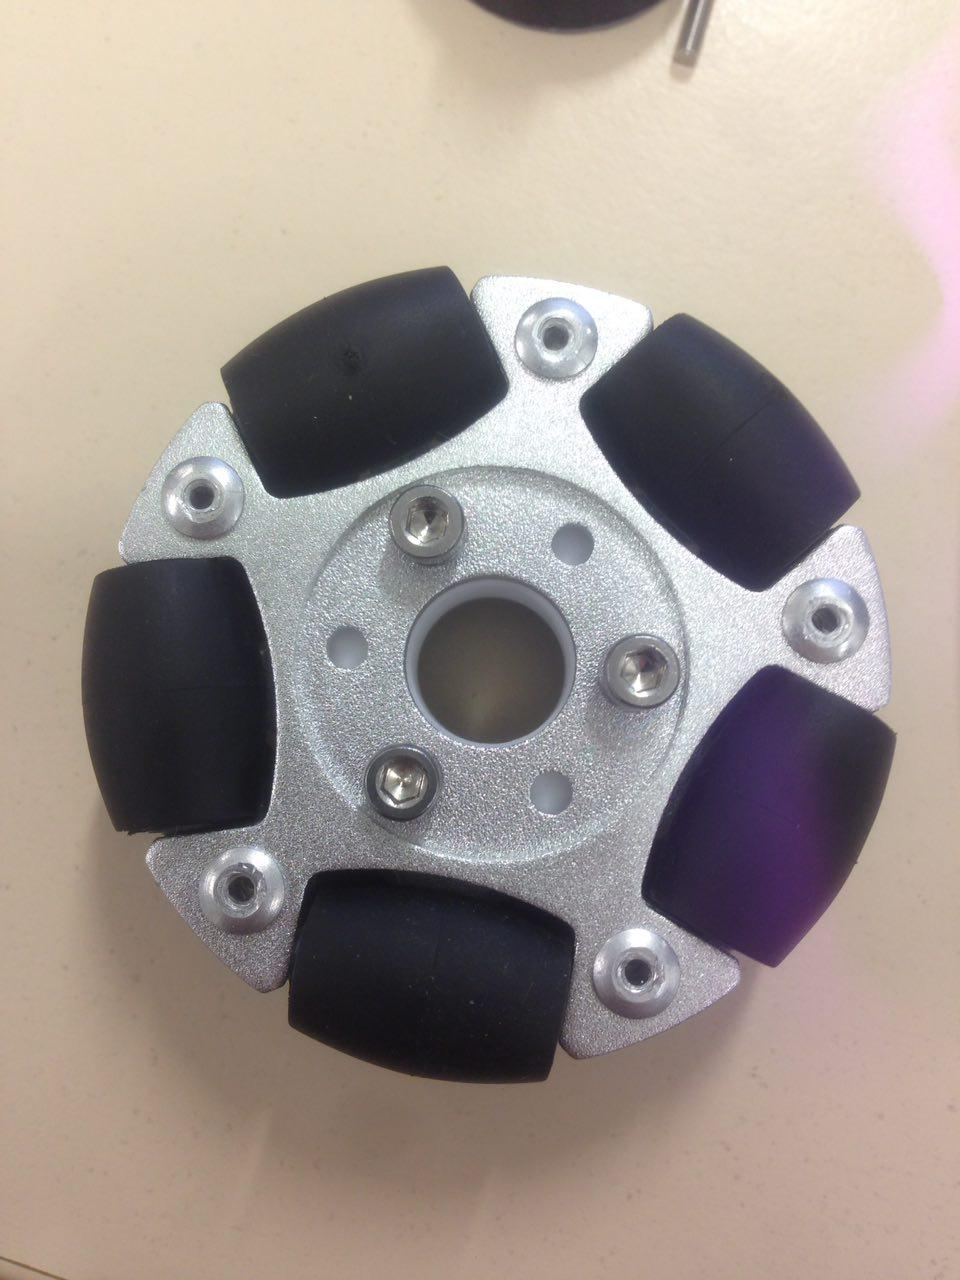
\includegraphics[width=0.05\textwidth]{./Bilder/Markus/img/wheel_double.jpg}\\
	
	Mitnehmer double wheels&3&7 & &  	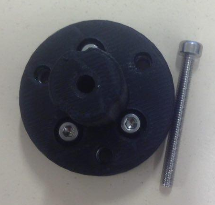
\includegraphics[width=0.05\textwidth]{./Bilder/Markus/img/mitnehmer_double.png}   \\
	
	Ball(alum., dia.: 140mm, material thickness 2.5mm)&1&400&\mylink{http://www.ball-tech.de/Hohlkugeln/Aluminium/}{ball-tech gmbh,\EUR{40}. } & 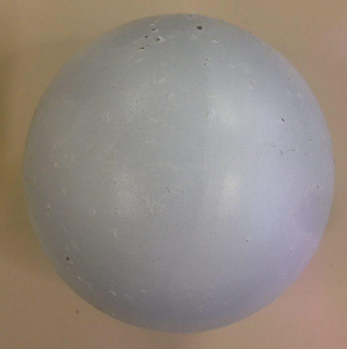
\includegraphics[width=0.1\textwidth]{./Bilder/Markus/img/white_ball.png}\\
	
	Ball(gummi, diameter: 150mm)&1&326&link and cost&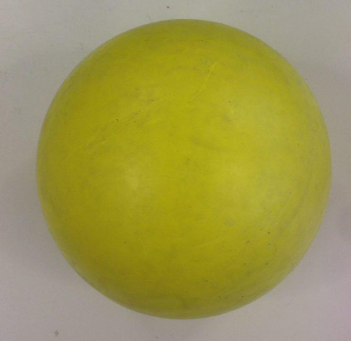
\includegraphics[width=0.1\textwidth]{./Bilder/Markus/img/yellow_ball.png}\\	
\end{tabular}
\end{table}

Die Gesamtkosten der verwendeten Bauteile belief sich auf ca. \EUR{1200}.

\chapter{ROS-Graph Simulation} \label{fig:rosgraph}
\begin{figure}[htbp]%
	{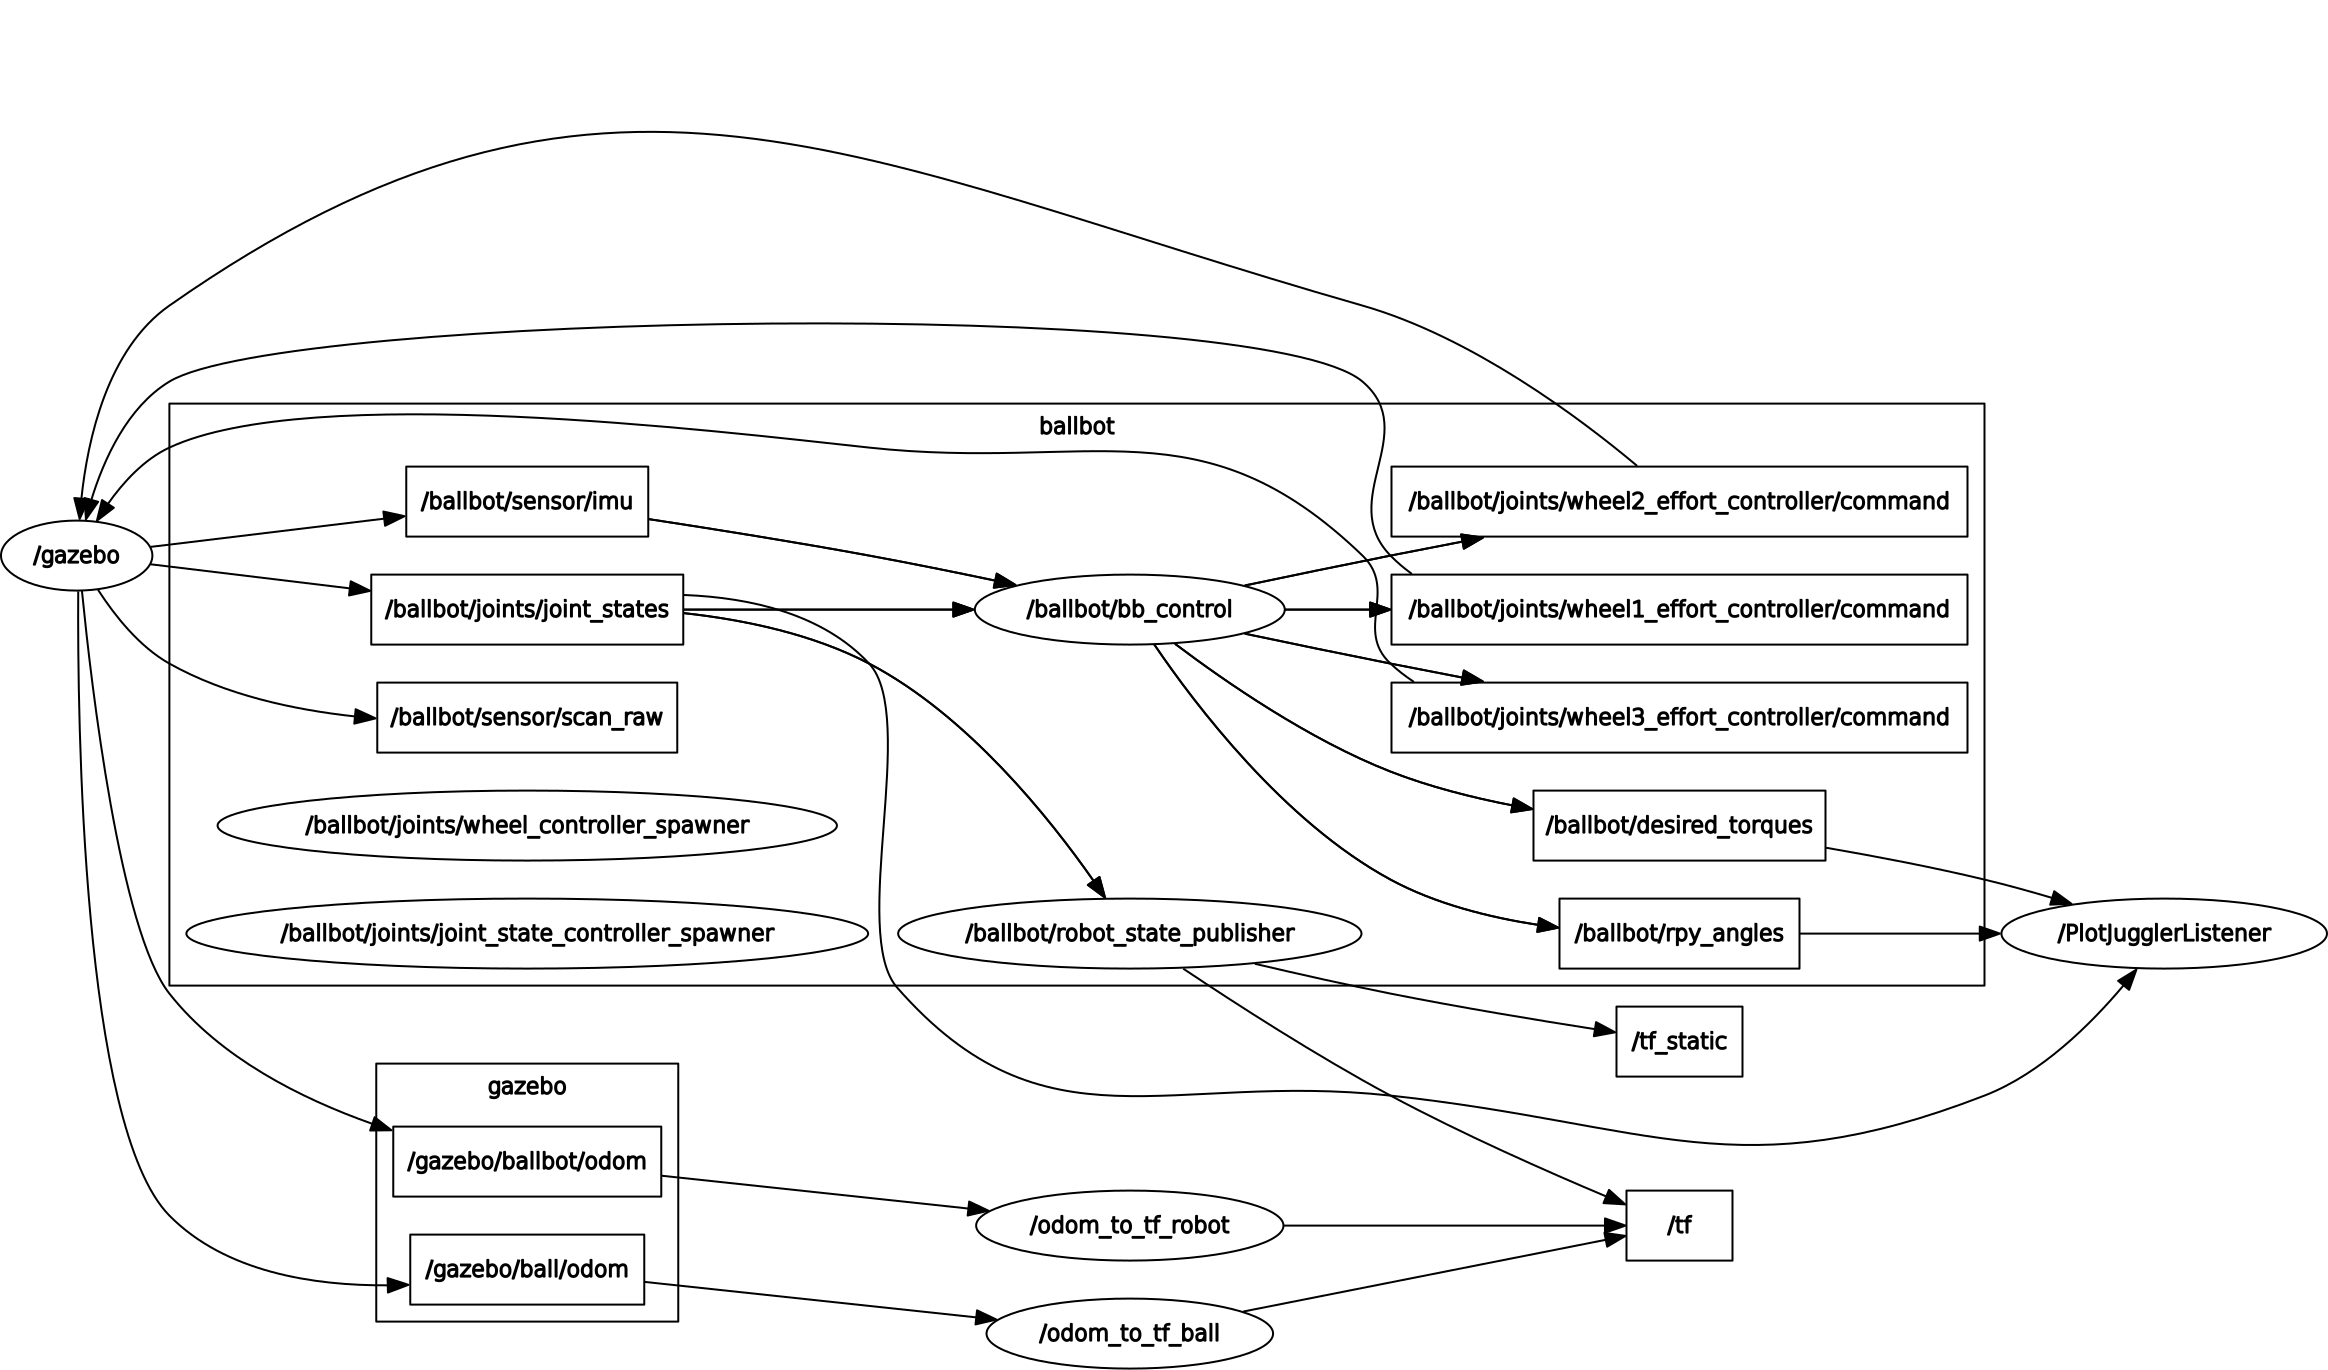
\includegraphics[scale=0.25, angle=90]{./Bilder/Markus/rosgraph.png} }
	\caption{�bersicht aller Teilprogramme(Nodes) und deren Topics, die beim Starten der Simulation aktiv sind und Nachrichten austauschen. Hierbei sind die Nodes mit Ellipsen und die Topics mit Rechtecken gekennzeichnet. Das Bild wurde mit dem ROS Programm rqt\_graph erstellt.}
\end{figure}

\chapter{Simulink Simulationsaufbau} \label{ch:gesamtbild}
\begin{figure}[htbp]%
	{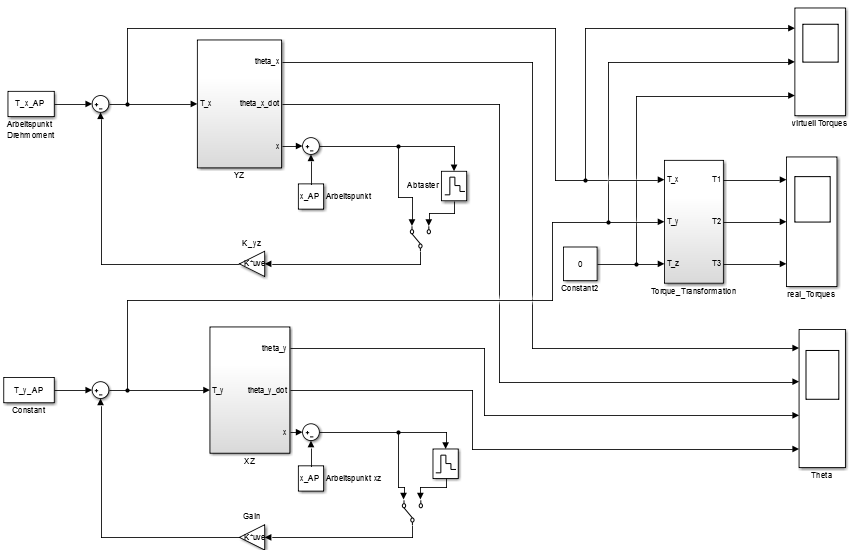
\includegraphics[scale=0.8, angle=90]{./Bilder/Florian/Komplett_System_MATLAB_SIMULINK.PNG} }
	\caption{�bersicht des Simulink Simulationsaufbaus}
\end{figure}
